%--------------------------------------------------------------------------------------------------------------------------------%
% Code and text for "A comparative test of the role of population structure in determining pathogen richness"
% Chapter 2 of thesis "The role of population structure and size in determining bat pathogen richness"
% by Tim CD Lucas
%
% NB The file is numbered Chapter3 as this was previously Chapter 3 in the thesis.
%
%---------------------------------------------------------------------------------------------------------------------------------%














\section{Abstract}


%\tmpsection{One or two sentences providing a basic introduction to the field}
% comprehensible to a scientist in any discipline.
\lettr{Z}oonotic diseases make up the majority of human infectious diseases and are a major drain on healthcare resources and economies.
Species that host many pathogen species are more likely to be the source of a novel zoonotic disease than species with few pathogens.
However, the factors that influence pathogen richness in animal species are poorly understood.
%
%
%\tmpsection{Two to three sentences of more detailed background}
% comprehensible to scientists in related disciplines.
% Theory led.
The pattern of contacts between individuals (i.e.\ population structure) can be influenced by habitat fragmentation, sociality and dispersal behaviour.
Epidemiological theory suggests that increased population structure can promote pathogen richness by reducing competition between pathogen species.
Conversely, it is often assumed that as greater population structure slows the spread of a new pathogen, less structured populations should have greater pathogen richness.
%
%
%\tmpsection{One sentence clearly stating the general problem (the gap)}
% being addressed by this particular study.
Previous studies have had contradictory results and different measures of population structure have been used, complicating the interpretation.
%
%
%\tmpsection{One sentence summarising the main result}
%  (with the words “here we show” or their equivalent).
Here I used comparative data across 203 bat species, controlling for body mass, range size, study effort and phylogeny, to test whether increased population structure correlates with viral richness.
Bats, as a group, make a useful case study because they have been associated with a number of important, recent zoonotic outbreaks.
Unlike previous studies, I used two measures of population structure: the number of subspecies and effective levels of gene flow.
I find that both measures are positively associated with pathogen richness.
%
%
%\tmpsection{Two or three sentences explaining what the main result reveals in direct comparison to what was thoughts to be the case previously}
% or how the main result adds to previous knowledge
My results add more robust support to the hypothesis that increased population structure promotes viral richness in bats.
The results support the prediction that increased population structure allows greater pathogen richness by reducing competition between pathogens
The prediction that factors that increase $R_0$ should increase pathogen richness is not supported.
%
%
%\tmpsection{One or two sentences to put the results into a more general context.}
Although my analysis implies that increased population structure does promote pathogen richness in bats, the weakness of the relationship and the difficulty in obtaining some measurements means that this is probably not a useful, predictive factor on its own for optimising zoonotic surveillance.
%However, the relationship has implications for global change, implying that increased habitat fragmentation might promote greater viral richness in bats.





%%%%%%%%%%%%%%%%%%%%%%%%%%%%%%%%%%%%%%%%%%%%%%%%%%%%%%%%%%%%%%%%%%%%%%%%%%%%%%%%%%%%%%%%%%%%%%%%%%%%%%%%%%%%%%%%%%%%%%%%%%%%%%%%%%%%%%%%%%%%%%%%%%%%%%%%%%%

\section{Introduction}

%%%%%%%%%%%%%%%%%%%%%%%%%%%%%%%%%%%%%%%%%%%%%%%%%%%%%%%%%%%%%%%%%%%%%%%%%%%%%%%%%%%%%%%%%%%%%%%%%%%%%%%%%%%%%%%%%%%%%%%%%%%%%%%%%%%%%%%%%%%%%%%%%%%%%%%%%%%

%#the introduction is not bad and starts very well but i think you need a bit more from studies of other mammals (not bats) to put the study into context as well as explaining why particularly you focus on pop structure, some justification of why bats, and less detail about the specific Fst measures (move to methods) and more stuff on your actual methods and approach you use in this study.

%#Structure could be:
%#1. Zoonotic disease is bad (as you have written it already)
%#2. Need to understand why some species have more pathogens than others. Life history variables of the host have been used to explain why some species have more than others, such as blah blah. However, pop structure (explain what this means) is of particular interest because of blah blah.
%#3. Epidemiological theoretical models predict relationship with pop structure and translated into across species patterns as increased structure less pathogen diversity but problem is of inter-pathogen competition
%#4. lack of large across species studies of these relationships - those that have been done have conflicting patterns (examples across different taxa).
%#5. Bats are very interesting in this regard because of blah
%#6. Bat studies of pathogen richness and population structure are particularly interesting in this area but also are conflicting (examples), due in part to low sample sizes and problems with comparing results using different definitions of population structure and not controlling for effects of phylogeny.
%#7. Here I use a phylogenetic comparative approach to understand the relationship between pop structure and pathogen richness across the largest study of bats to date. I use a phylogenetic GLM controlling for the other life history characteristics known to impact pathogen richness to quantify the relationship between viral richness (as a proxy for pathogen richness_ and two measures of population structure. 
%#8. I found ...

\tmpsection{General Intro}

%#1. Zoonotic disease is bad (as you have written it already)
Zoonotic pathogens make up the majority of newly emerging diseases and have profound consequences for public health, economics and international development \cite{jones2008global, smith2014global, ebolaWorldbank}.
Better models for predicting which wild host species are potential reservoirs of zoonotic diseases would allow us to optimise zoonotic disease surveillance and anticipate how the risks of disease spillover might change with global change.
The chance that a host species will be the source of an outbreak depends on a number of factors, such as its proximity and interactions with humans, and the prevalence and the number of pathogen species it carries \cite{wolfe2000deforestation}.
However, the factors that control the number of pathogen species in a host species remain poorly understood.


\tmpsection{Specific Intro}

%#2. Need to understand why some species have more pathogens than others. Life history variables of the host have been used to explain why some species have more than others, such as blah blah. 
\tmpsection{Theoretical background}


A number of species traits that might control pathogen richness have been studied.
These traits can be at the level of the individual (e.g., body mass and longevity) or the level of the population (e.g., population density, sociality and species range size).
Large bodied animals have been shown to have high pathogen richness with large bodies providing more resources for pathogens \cite{kamiya2014determines, arneberg2002host, poulin1995phylogeny, bordes2008bat, luis2013comparison}.
Long lived species are expected to have high pathogen richness, because the number of pathogens a host encounters in its lifetime will be higher \cite{nunn2003comparative, ezenwa2006host, luis2013comparison}.
Animal density \cite{kamiya2014determines, nunn2003comparative, arneberg2002host} and sociality \cite{bordes2007rodent, vitone2004body, altizer2003social, ezenwa2006host} are both predicted to increase pathogen richness by increasing the rate of spread, $R_0$, of a new pathogen.
Finally, widely distributed species have high pathogen richness, potentially because they experience a wider range of environments or because they are sympatric with more species \cite{kamiya2014determines, nunn2003comparative, luis2013comparison}.

%# However, pop structure (explain what this means) is of particular interest because of blah blah.

%#3. Epidemiological theoretical models predict relationship with pop structure and translated into across species patterns as increased structure less pathogen diversity but problem is of inter-pathogen competition


A further population level factor that may affect pathogen richness is population structure.
Population structure can be defined as the extent to which interactions between individuals in a population are non-random.
The role of population structure on human epidemics has been studied in depth and it has been shown that decreased population structure increases the speed of pathogen spread and makes establishment of a new pathogen more likely \cite{colizza2007invasion, vespignani2008reaction}.
In comparative studies of pathogen richness in wild animals, this relationship with $R_0$ is often taken as a prediction that decreased population structure will increase pathogen richness relative to other host species \cite{nunn2003comparative, morand2000wormy, poulin2014parasite, poulin2000diversity, altizer2003social}. 
However, epidemiological models of highly virulent pathogens have shown that increased population structure can allow persistence of a pathogen where a well-mixed population would experience a single, large epidemic followed by pathogen extinction \cite{blackwood2013resolving, plowright2011urban}.
Furthermore, the assumption that high $R_0$ leads to high pathogen richness ignores inter-pathogen competition.
Simple epidemiological models of competition between multiple pathogens show that, in completely unstructured populations, a competitive exclusion process occurs but that adding population structure makes coexistence possible \cite{qiu2013vector, allen2004sis, nunes2006localized}.


\tmpsection{Previous Studies}

%#4. lack of large across species studies of these relationships - those that have been done have conflicting patterns (examples across different taxa).

There is a lack of large, comparative studies of the role of population structure on pathogen richness.
Sociality, which is one constituent part of population structure, has been well studied.
However, in primates only a weak positive association between sociality and pathogen richness was found \cite{vitone2004body}.
Furthermore, a negative association was found in rodents \cite{bordes2007rodent} and in even and odd-toed hoofed mammals \cite{ezenwa2006host}.
Finally, two studies tested for an association between group size and parasite richness in bats \cite{bordes2008bat, gay2014parasite}.
Amongst 138 bat species, \textcite{bordes2008bat} found no relationship between group size (coded into four classes) and bat fly species richness.
\textcite{gay2014parasite} a negative relationship between colony size and viral richness but a positive relationship between colony size and ectoparasite richness.
While sociality is an important component of population structure it does not capture fully how connected the population is globally. 


%#5. Bats are very interesting in this regard because of blah

%#6. Bat studies of pathogen richness and population structure are particularly interesting in this area but also are conflicting (examples), due in part to low sample sizes and problems with comparing results using different definitions of population structure and not controlling for effects of phylogeny.


Three studies have used comparative data to test for an association between global population structure and viral richness in bats.
A study on 15 African bat species found a positive relationship between the extent of distribution fragmentation and viral richness \cite{maganga2014bat}.
Conversely, a study on 20 South-East Asian bat species found the opposite relationship \cite{gay2014parasite}. 
These studies used the ratio between the perimeter and area of the species' geographic range as their measure of population structure.
However, range maps are very coarse for many species.
Furthermore, range maps are likely to be more detailed (and therefore have a greater perimeter) in well studied species.

A global study on 33 bat species found a positive relationship between $F_{ST}$ --- a measure of genetic structure --- and viral richness \cite{turmelle2009correlates}. 
However, this study included measures using mtDNA which only measures female dispersal which may have biased the results as many bat species show female philopatry \cite{kerth2002extreme, hulva2010mechanisms}.
Furthermore, this study used measures of $F_{ST}$ irrespective of the spatial scale of the study including studies covering from tens \cite{mccracken1981social} to thousands \cite{petit1999male} of kilometres.
As isolation by distance has been shown in a number of bat species \cite{burland1999population, hulva2010mechanisms, o2015genetic, vonhof2015range}, this could bias results further.
Finally, when a global $F_{ST}$ value is not given, \textcite{turmelle2009correlates} used the mean of all pairwise $F_{ST}$ values between sites.
This is not correct as pairwise and global $F_{ST}$ values have different relationships with effective migration rates. 



\tmpsection{The gap}
\tmpsection{What I did/found}

%#7. Here I use a phylogenetic comparative approach to understand the relationship between pop structure and pathogen richness across the largest study of bats to date. I use a phylogenetic GLM controlling for the other life history characteristics known to impact pathogen richness to quantify the relationship between viral richness (as a proxy for pathogen richness_ and two measures of population structure. 
%#8. I found ...

Here I used a phylogenetic comparative approach to test for a relationship between increased population structure and pathogen richness in the largest study of bats to date. 
I used phylogenetic linear models, controlling for the other life history characteristics known to impact pathogen richness, to quantify the relationship between viral richness (as a proxy for pathogen richness) and two measures of population structure: the number of subspecies and effective gene flow. 
I used two measures of population structure to increase the robustness of the analysis; this is particularly important as previous studies have had contradictory results \cite{maganga2014bat, gay2014parasite, turmelle2009correlates}.

I found that increases in both measures of population structure are positively associated with viral richness and are included as explanatory variables in the best models for describing viral richness.
Furthermore, I found that the role of phylogeny is very weak both in the models and in the distribution of viral richness amongst taxa.


%%%%%%%%%%%%%%%%%%%%%%%%%%%%%%%%%%%%%%%%%%%%%%%%%%%%%%%%%%%%%%%%%%%%%%%%%%%%%%%%%%%%%%%%%%%%%%%%%%%%%%%%%%%%%%%%%%%%%%%%%%%%%%%%%%%%%%%%%%%%%%%%%%%%%%%%%%%

\section{Methods}

%%%%%%%%%%%%%%%%%%%%%%%%%%%%%%%%%%%%%%%%%%%%%%%%%%%%%%%%%%%%%%%%%%%%%%%%%%%%%%%%%%%%%%%%%%%%%%%%%%%%%%%%%%%%%%%%%%%%%%%%%%%%%%%%%%%%%%%%%%%%%%%%%%%%%%%%%%%


\subsection{Data Collection}

\subsubsection{Pathogen richness}

To measure pathogen richness I used data from \textcite{luis2013comparison}. 
This data simply includes known infections of a bat species with a virus species. 
I have used viral richness as a proxy for pathogen richness more generally, but the analysis could also be considered as representative of viral richness only.
Rows with host species that were not identified to species level according to \textcite{wilson2005mammal} were removed.
Many viruses were not identified to species level or their specified species names were not in the ICTV virus taxonomy \cite{ICTV}.
Therefore, I counted a virus if it was the only virus, for that host species, in the lowest taxonomic level identified (present in the ICTV taxonomy).
For example, if a host is recorded as harbouring an unknown Paramyxoviridae virus, then it is logical to assume that the host carries at least one Paramyxoviridae virus.
If a host carries an unknown Paramyxoviridae virus and a known Paramyxoviridae virus, it is hard to confirm that the unknown virus is not another record of the known virus.
In this case, the host would be counted as having one virus species.


%$F_{ST}$ studies are conducted at a range of spatial scales, but $F_{ST}$ often increases with distance studied \cite{burland1999population, hulva2010mechanisms, o2015genetic, vonhof2015range}.
%To minimise the effects of this I only used data from studies that cover rangeUseable * 100\% of the diameter of the species range.
%This is a largely arbitrary value that could be considered to reflect a ``global'' estimate of $F_{ST}$ while keeping a reasonable number of data points available.
%I calculated the diameter of the species range by finding the furthest apart points in the IUCN species range \cite{iucn} even if the range is split into multiple polygons.
%The width covered by each study was the distance between the most distant sampling sites.
%When this was not explicit in the paper, the centre of the lowest level of geographic area was used.





















































































		
























%%%%%%%%%%%%%%%%%%%%%%%%%%%%%%%%%%%%%%%%%%%%%%%%%%%%%%%%%%%%%%%%%%%%%%%%%%%%%%%%%%%%%%%%%%%%%%%%%%%%%%%%%%%%%%%%%%%%%%%%%%%%%%%%%%%%%%%%%%%%%%%%%%%%%%%%%%%
%%%% FST ANALYSIS                                                                                                                                  %%%%%%%%
%%%%%%%%%%%%%%%%%%%%%%%%%%%%%%%%%%%%%%%%%%%%%%%%%%%%%%%%%%%%%%%%%%%%%%%%%%%%%%%%%%%%%%%%%%%%%%%%%%%%%%%%%%%%%%%%%%%%%%%%%%%%%%%%%%%%%%%%%%%%%%%%%%%%%%%%%%%
































































\subsubsection{Population structure data}

I used two measures of population structure: the number of subspecies and the effective level of gene flow.
The number of subspecies was counted using the taxonomy from \textcite{wilson2005mammal}.
The effective level of gene flow was calculated from estimates of $F_{ST}$ collated from the literature.
The studies were from a wide range of spatial scales, from local ($\sim\SI{10}{\kilo\metre}$) to continental.
As $F_{ST}$ often increases with spatial scale \cite{burland1999population, hulva2010mechanisms, o2015genetic, vonhof2015range} I controlled for this by only using data from studies where a large proportion of the species range was studied.
I used the ratio of the furthest distance between $F_{ST}$ samples (taken from the paper or measured with \url{http://www.distancefromto.net/} if not stated) to the length of the IUCN species range \cite{iucn} and only used studies if this ratio was greater than 0.2.
This is an arbitrary value that was a compromise between retaining a reasonable number of data points and controlling for the bias in spatial scale.
I only used global $F_{ST}$ estimates as the mean of pairwise $F_{ST}$ values is not necessarily equal to the global $F_{ST}$ value.
I converted all $F_{ST}$ values to effective migration rates using $M = (1-F_{ST})/4F_{ST}$.
This transforms the data from being bound by $(0, 1)$ to being in the range $\lbrack 0, \infty)$ and is easier to interpret. 

The two measures of population structure were analysed separately because the number of subspecies data set had 196 data points but there was only $F_{ST}$ data for 24 bat species.
For the subspecies analysis, all bat species in \textcite{luis2013comparison} were used (i.e.\ all species with at least one known virus species).
This was to avoid using the very large number of bat species that have simply never been sampled for viruses.
However, for the gene flow analysis, all bat species with suitable $F_{ST}$ estimates were used.
As some bat species had suitable $F_{ST}$ estimates but were not present in \textcite{luis2013comparison}, some bat species with zero known virus species were included. 
These bat species with no known viruses were included to make the greatest use of the $F_{ST}$ data available and because the number of species with no known virus species was not unduly large (7 species).

After data cleaning there was data for 196 bat species in 11 families for the subspecies analysis.
Due to the limited number of studies and the restrictive requirements imposed on study design, there was only data for 24 bat species in 7 families for the effective gene flow analysis.
The raw data are included in Table \ref{A-rawData}.




\subsubsection{Other explanatory variables}



To control for study bias I collected the number of PubMed and Google Scholar citations for each bat species name including synonyms from ITIS \cite{itis} via the \emph{taxize} package \cite{chamberlain2013taxize}.
The counts were scraped using the \emph{rvest} package \cite{rvest}.
I log transformed these variables as they were strongly right skewed.
I tested for correlation between these two proxies for study effort using phylogenetic least squares regression (pgls), using the best-supported phylogeny from \textcite{fritz2009geographical}, and likelihood ratio tests using the \emph{caper} package \cite{caper} (Figures~\ref{fig:treePlot} and \ref{fig:scholarvspubmedPlot}).
The log number of citations on PubMed and Google scholar were highly correlated (pgls: $t$ = 19.32, df = 194, $p < 10^{-5}$).
As the correlation between citation counts is strong, I only used Google Scholar reference counts in subsequent analyses.
%See the appendix for analyses run using PubMed citations.

A number of other factors that have previously been found to be important were included as additional explanatory variables: body mass \cite{kamiya2014determines, turmelle2009correlates, gay2014parasite, maganga2014bat, han2015infectious, bordes2008bat}, range size \cite{kamiya2014determines, turmelle2009correlates, maganga2014bat}.		
These other factors were included to avoid spurious positive results occurring simply due to correlations between pathogen richness and a different, causal factor.
Despite commonly being associated with pathogen richness \cite{arneberg2002host, kamiya2014determines, nunn2003comparative}, population density is not included in the analysis as there is very little data for bat densities.
Measures of body mass were taken from Pantheria \cite{jones2009pantheria} and primary literature \cite{canals2005relative, arita1993rarity, lopez2014echolocation, orr2013does, lim2001bat, aldridge1987turning, ma2003dietary, owen2003home, henderson2008movements, heaney2012nyctalus, oleksy2015high, zhang2009recent}. 
\emph{Pipistrellus pygmaeus} was assigned the same mass as \emph{P. pipistrellus} as they are indistinguishable by mass.
Body mass measurements were log transformed as they were strongly right skewed.
Distribution size was estimated by downloading range maps for all species from IUCN \cite{iucn} and were also log transformed due to right skew.




\subsection{Statistical analysis}

Statistical analysis for both response variables --- number of subspecies and effective level of gene flow --- was conducted using an information theoretical approach \cite{burnham2002model}, specifically following \textcite{whittingham2005habitat, whittingham2006we}.
All analysis were performed in R \cite{R} and all code is available on \url{https://github.com/timcdlucas/PhDThesis/blob/master/Chapter3.Rtex}.
I chose a credible set of models including all combinations of explanatory variables and a model with just an intercept.
In the analysis using the number of subspecies response variable I also modelled the interaction study effort and number of subspecies by including their product.
This interaction was included as I believed \emph{a priori} that this interaction may be present as subspecies in well studied species are more likely to be identified.
The interaction was only included in models with both study effort and number of subspecies as individual terms.
Following \textcite{whittingham2005habitat} I included a uniformly distributed random variable.
This variable can be used to benchmark how important other explanatory variables are.
The whole analysis was run 50 times, resampling the random variable each time.


To control for phylogenetic non-independence of datapoints I used the best-supported phylogeny from \textcite{fritz2009geographical} (Figure~\ref{fig:treePlot}) which is the supertree from \textcite{bininda2007delayed} with names updated to match the taxonomy by \textcite{wilson2005mammal}.
Phylogenetic manipulation was performed using the \emph{ape} package \cite{ape}.
I also performed the analysis using the phylogeny from \textcite{jones2005bats} as this has some broad topological differences including the Rhinolophoidea being sister to the Pteropodidae rather than being related to the other insectivorous bats (Figure~\ref{fig:treePlot2}). 






\begin{knitrout}\footnotesize
\definecolor{shadecolor}{rgb}{0.969, 0.969, 0.969}\color{fgcolor}\begin{figure}[t]

{\centering 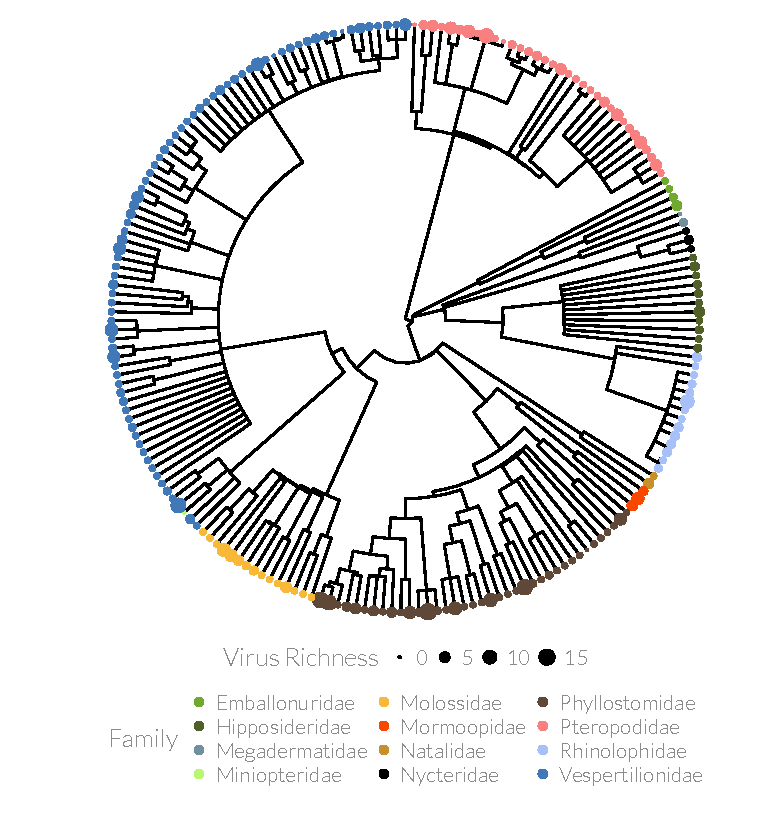
\includegraphics[width=1\textwidth,trim = 0cm 0cm 0cm 0cm]{figure/treePlot-1} 

}

\caption[Pruned phylogeny with dot size showing number of pathogens and colour showing family.]{
The phylogenetic distribution of viral richness.
There is no clear association between phylogeny and virus richness (pgls: $\lambda =$ 0.04, $p =$ 0.21).
The phylogeny is from \cite{bininda2007delayed} pruned to include all species used in either the number of subspecies or gene flow analysis.
Dot size shows the number of known viruses for that species and colour shows family.
The red scale bar shows 25 million years.}\label{fig:treePlot}
\end{figure}


\end{knitrout}



The importance of the phylogeny on each variable separately was examined by estimating the $\lambda$ parameter when regressing the variable against an intercept using the \emph{pgls} function in \emph{caper} \cite{caper}.
The parameter $\lambda$ usually takes values between zero and one and \emph{pgls} constrains $\lambda$ within these bounds. 
$\lambda = 0$ implies no autocorrelation while a trait evolving by Brownian motion along the tree would have $\lambda = 1$.
I tested fitted $\lambda$ values against the null hypothesis of $\lambda = 0$ (no correlation between species) with log-likelihood ratio tests using \emph{caper} \cite{caper}.

I fitted phylogenetic regressions for all models in the credible set using the function \emph{gls} in the package \emph{nlme} \cite{nlme}.
The explanatory variables were centred and scaled to allow direct comparison of the coefficients \cite{schielzeth2010simple}.
For each regression model I simultaneously fitted the $\lambda$ parameter as this avoids misspecifying the model \cite{revell2010phylogenetic}.
Unlike the \emph{pgls} function, \emph{gls} does not constrain $\lambda$ to be in the range $\lbrack 0, 1\rbrack$.
$\lambda < 0$ indicates that residuals from the fitted model are distributed on the phylogeny more uniformly than expected by chance.
$\kappa$ and $\delta$ parameters were constrained to one as they are more concerned with when along a branch evolution occurs than the importance of the phylogeny.
Further, fitting multiple parameters makes interpretation difficult. 


To establish the importance of variables I calculated the probability, $Pr$, that each variable would be in the best model amongst those examined (under the assumption that all models are \emph{a priori} equally likely).
This value can more generally, and with fewer assumptions, be considered as simply the relative weight of evidence for each variable being in the best model amongst those examined.
I calculated AICc for each model.
I calculated the average AICc, $\bar{\text{AICc}}$, by averaging AICc scores within models.
$\Delta\text{AICc}$ was calculated as $\text{min}(\bar{\text{AICc}}) - \bar{\text{AICc}}$, not the mean of the individual $\Delta\text{AICc}$ scores, to guarantee that the best model has $\Delta\text{AICc} = 0$.
From these $\Delta\text{AICc}$ values I calculated Akaike weights, $w$.
This value can be interpreted as the probability that a model is the best model, given the data, amongst those examined.
For each variable, the sum of the Akaike weights of models containing that variable are summed to give $Pr$.
This value can be interpreted as the probability that the given variable is in the best model.

To determine the direction and strength of the effect of each variable the mean of its regression coefficient, $b$, in all models that contained that variable, weighted by the model's Akaike weight, was also calculated.
In the subspecies analysis the inclusion of an interaction term between number of subspecies and study effort makes interpretation of this mean coefficient more difficult, particularly because the interaction term greatly affects the estimated value of $b$.
To aid interpretation, the mean coefficient for the number of subspecies was calculated for: \emph{i}) all models containing the number of species, \emph{ii}) only models with the interaction term and \emph{iii}) only models with the number of subspecies but not the interaction term.






		
\begin{knitrout}\footnotesize
\definecolor{shadecolor}{rgb}{0.969, 0.969, 0.969}\color{fgcolor}\begin{figure}[t]

{\centering 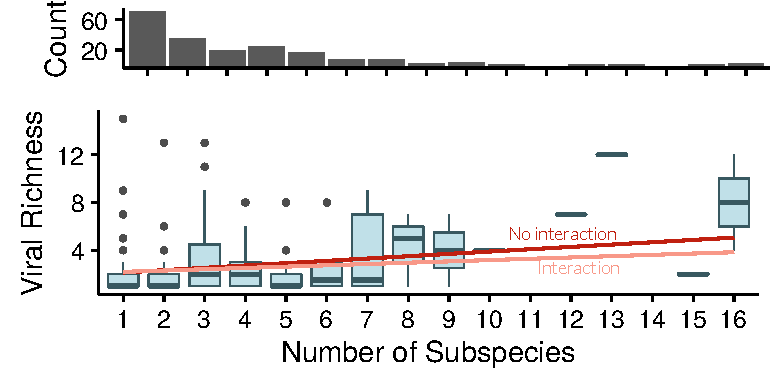
\includegraphics[width=0.8\textwidth]{figure/boxplot-1} 

}

\caption[The relationship between number of subspecies and viral richness for 196 bat species.]{The relationship between number of subspecies and viral richness for 196 bat species.
The area of the circle shows the number of bat species at each discrete value.
48 bat species have one subspecies and one known virus species.
The red line represents a phylogenetic multiple regression including all the explanatory variables but no interaction term.
The line shows the slope from the multiple regression with the intercept being calculated by setting other explanatory variables to their median values.
}\label{fig:boxplot}
\end{figure}


\end{knitrout}


%%%%%%%%%%%%%%%%%%%%%%%%%%%%%%%%%%%%%%%%%%%%%%%%%%%%%%%%%%%%%%%%%%%%%%%%%%%%%%%%%%%%%%%%%%%%%%%%%%%%%%%%%%%%%%%%%%%%%%%%%%%%%%%%%%%%%%%%%%%%%%%%%%%%%%%%%%%

\section{Results}

%%%%%%%%%%%%%%%%%%%%%%%%%%%%%%%%%%%%%%%%%%%%%%%%%%%%%%%%%%%%%%%%%%%%%%%%%%%%%%%%%%%%%%%%%%%%%%%%%%%%%%%%%%%%%%%%%%%%%%%%%%%%%%%%%%%%%%%%%%%%%%%%%%%%%%%%%%%



\subsection{Number of Subspecies}
\tmpsection{More descriptive}

The number of described virus species for a bat host ranged up to 15 viruses in \emph{Carollia perspicillata}.
There appears to be a positive relationship between the number of subspecies and viral richness (Figure~\ref{fig:boxplot}) though few species have more than five subspecies. 
Out of 39 fitted models, the top seven models all had $\Delta\text{AICc} < 4$ meaning there was no clear best model (Table~\ref{t:models} and Table \ref{A-modelWeights}).
However these top seven models all contained study effort, number of subspecies and the interaction between these two variables.
The explanatory variables log(Mass), log(Range Size) and the uniformly random variable are each in three of the top seven models.
These top seven models had a combined weight of 0.96 meaning that there is a 96\% chance that one of these models is the best model amongst those examined.



Summing the Akaike weights of all models that contain a given variable gives a probability, $Pr$, that the variable would be in the best model amongst those in the plausible set \cite{whittingham2006we}.
The number of subspecies is very likely in the best model ($Pr > $ 0.99) as is the interaction term between the number of subspecies and study effort ($Pr = $ 0.96) compared to the benchmark random variable which has $Pr = $ 0.25 (Figure~\ref{fig:fstITPlots}A and Table~\ref{t:variables}).
When models with the interaction term are removed there is, on average (mean weighted by Akaike weights), a positive relationship between the number of subspecies and viral richness ($b = $ 0.63, variance = 0.02).
Models with an interaction term between the number of subspecies and study effort have a positive interaction term ($b = $ 0.5, variance = \ensuremath{5.11\times 10^{-5}}) and linear term ($b = $ 0.31, variance = \ensuremath{2.13\times 10^{-4}}).








\begin{knitrout}\footnotesize
\definecolor{shadecolor}{rgb}{0.969, 0.969, 0.969}\color{fgcolor}\begin{figure}[t]

{\centering 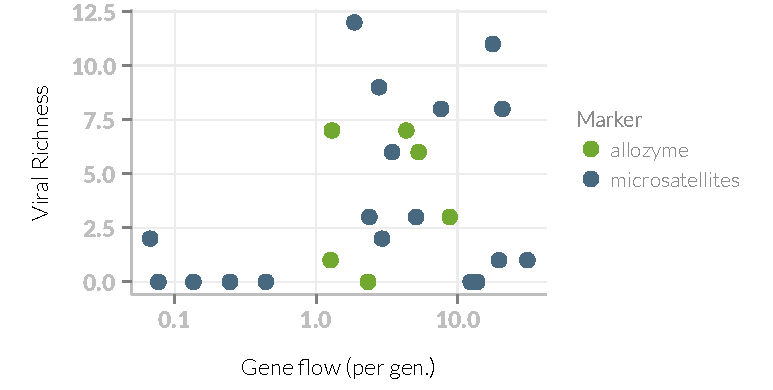
\includegraphics[width=0.8\textwidth]{figure/fstRawData-1} 

}

\caption[Relationship between viral richness and log effective gene flow per generation for 24 bat species.
]{Relationship between viral richness and log effective gene flow per generation for 24 bat species.
Green points are studies that estimated effective gene flow using allozymes and blue points are studies using microstatellites.
}\label{fig:fstRawData}
\end{figure}


\end{knitrout}




Study effort is very likely in the best model ($b = $ 0.99, $Pr > $ 0.99).
Body mass and range size are also probably in the best model ($b = $ 0.48, $Pr = $ 0.73 and $b = $ 0.35, $Pr = $ 0.54 respectively) with positive relationships of slightly lower strength than the number of subspecies in models without an interaction term ($b = $ 0.63, variance = 0.02).	


When using the phylogeny from \textcite{jones2005bats} the results are broadly similar (Figure~\ref{f:A-itplots} and Tables~\ref{A-modelWeights2} and \ref{t:variables2}).
Study effort, the number of subspecies and the interaction between the number of subspecies and study effort have strong support while range size and mass have intermediate support.
However, mass, range size and the interaction between number of subspecies and study effort have slightly weaker support than in the analysis using the phylogeny from \textcite{bininda2007delayed}.




\begin{knitrout}\footnotesize
\definecolor{shadecolor}{rgb}{0.969, 0.969, 0.969}\color{fgcolor}\begin{figure}[t]

{\centering 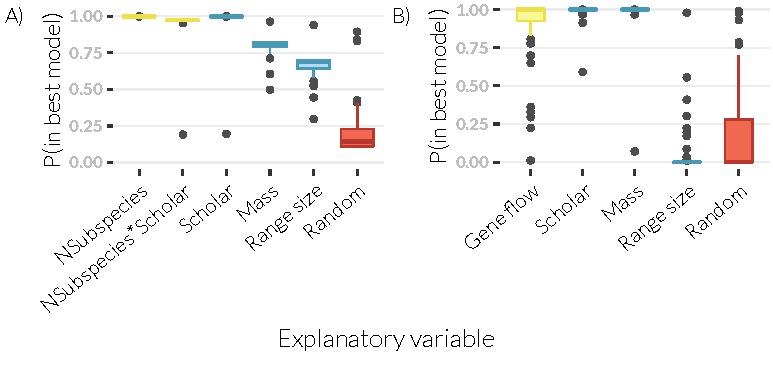
\includegraphics[width=\textwidth]{figure/fstITPlots-1} 

}

\caption[Akaike variable weights]{
The relative weight of evidence that each explanatory variable is in the best model for explaining viral richness.
The probability that each variable is in the best model (amongst the models tested) is shown for A) the number of subspecies analysis and B) the effective gene flow analysis.
The boxplots show the variation of the results over 50 resamplings of the uniformly random ``null'' variable. 
The thick bar of the boxplot shows the median value, the interquartile range is represented by a box, vertical lines represent range, and outliers are shown as filled circles.
The red ``Random'' box is the uniformly random variable. 
Population structure (number of subspecies and effective gene flow), shown in yellow, is likely to be in the best model in both analyses.}\label{fig:fstITPlots}
\end{figure}


\end{knitrout}

\tmpsection{Model results}




\subsection{Gene Flow}

\tmpsection{More Descriptive}

%Figure~\ref{fig:fstTreePlot} shows the phylogeny used and the number of viruses for each species.
The number of described virus species for a bat host ranged up to 12 viruses in \emph{Miniopterus schreibersii} (Figure~\ref{fig:fstRawData}).
Only the model with study effort, gene flow and body mass was well supported with the second model having an $\Delta\text{AICc}$ of 34 (Table \ref{t:models} and Table \ref{A-modelWeights}).
The effective level of gene flow was likely in the best model ($Pr > 0.999$, see Figure~\ref{fig:fstITPlots}B and Table~\ref{t:variables}).
On average (mean weighted by Akaike weights) there was a negative relationship between gene flow and viral richness ($b = $ \ensuremath{-0.67}, variance = \ensuremath{5.48\times 10^{-3}}) despite the insignificant positive relationship (Figure~\ref{fig:fstRawData}) estimated by the single-predictor model (pgls: $b$ = 0.63, $t$ = 1.16, df = 13, $p$ = 0.27).
Possibly due to the smaller sample size, or a weaker relationship, this coefficient was much more varied than the number of subspecies coefficient with 22\% of multiple-regression models estimating a positive relationship.

Study effort was very likely in the best model ($Pr > 0.999$) as was body mass ($Pr > 0.999$).
However, body mass had a negative average coefficient ($b = $ \ensuremath{-0.35}, variance = 0.04). % which is in contrast to the number of subspecies analysis, many studies in the literature \cite{kamiya2014determines, turmelle2009correlates, gay2014parasite, maganga2014bat} and the single-predictor model (pgls: $b$ = 0.6, $t$ = 0.38, df = 13, $p$ = 0.71).
In contrast to the number of subspecies analysis, range size was almost certainly not in the best model with $Pr = $ \ensuremath{3.96\times 10^{-8}}.
%This variable being less supported than the random variable may be because range size is closely correlated with study effort (pgls: $b$ = fstDistrStudyEffort$coefficients['log(distrSize)', 'Estimate'], $t$ = fstDistrStudyEffort$coefficients['log(distrSize)', 't value'], df = fstDistrStudyEffort$df[2], $p$ = fstDistrStudyEffort$coefficients['log(distrSize)', 'Pr(>|t|)']).
Of the three explanatory variables in the best model, study effort had the largest effect ($b = $ 2.49, variance = 0.08).
The effect size of gene flow ($b = $ \ensuremath{-0.67}, variance = \ensuremath{5.48\times 10^{-3}}) was approximately twice the size of that of body mass ($b = $ \ensuremath{-0.35}, variance = 0.04)



When using the phylogeny from \textcite{jones2005bats} the analysis became very unstable (Figure~\ref{f:A-itplots}).
The support for each variable changed dramatically with each resampling of the random variable.
On average however, only the model containing mass and range size is supported (Tables~\ref{A-fstModelWeights} and \ref{t:variables2}).



\afterpage{ % use after page to make sure this whole table is at the end of a page.
\begin{landscape}
\begin{table}[t]
\centering
%\rowcolors{2}{gray!25}{white}
\caption[Model selection results]{
Model selection results for number of subspecies and effective level of gene flow analysis. 
Models are ranked according to $\bar{\text{AICc}}$ and only the best nine and three  models are shown respectively.
Models were fitted to all combinations of variables (in total 39 number of subspecies models and 32 effective gene flow models).
$\bar{\text{AICc}}$ is the mean AICc score across 50 resamplings of the null random variable. 
$\Delta$AICc is the model's $\bar{\text{AICc}}$ score minus $\text{min}(\bar{\text{AICc}})$. 
$w$ is the Akaike weight and can be interpreted as the probability that the model is the best model (of those in the plausible set).
$\sum w$ is the cumulative sum of the Akaike weights.
log(Scholar)*NSubspecies indicates the interaction term between study effort and number of subspecies.
%In the number of subspecies analysis there are many models with low $\Delta$AICc scores suggesting there there is no single `best model'.
%In the gene flow analysis, only the top model is supported.
}


\begin{tabular}{@{}>{\footnotesize}lrrrr@{}}

\toprule
\normalsize{Model} & $\bar{\text{AICc}}$ & $\Delta$AICc & $w$ & $\sum w$\\
\midrule
&&&&\\[-3mm]
\textit{\small{Number of Subspecies}} &&&&\\
%1
log(Scholar) + NSubspecies + log(Scholar)*NSubspecies  + log(Mass) + log(RangeSize) & 
882 & 0.00 &
0.38 & 0.38\\
%2
log(Scholar) + NSubspecies + log(Scholar)*NSubspecies  + log(Mass) & 
884 & 1.39 &
0.19 & 0.57\\
%3
log(Scholar) + NSubspecies + log(Scholar)*NSubspecies + Random + log(Mass) & 
885 & 2.24 &
0.12 & 0.70\\
%4
log(Scholar) + NSubspecies + log(Scholar)*NSubspecies  & 
885 & 3.14 &
0.08 & 0.78\\
%5
log(Scholar) + NSubspecies + log(Scholar)*NSubspecies  + log(RangeSize) & 
886 & 3.18 &
0.08 & 0.86\\
%6
log(Scholar) + NSubspecies + log(Scholar)*NSubspecies  + Random + log(RangeSize) & 
886 & 3.94 &
0.05 & 0.91\\
%7
log(Scholar) + NSubspecies + log(Scholar)*NSubspecies  + Random & 
886 & 3.95 &
0.05 & 0.96\\
%8
log(Scholar) + NSubspecies + log(Mass) + Random & 
889 & 6.93 &
0.01 & 0.97\\
%9
log(Scholar) + NSubspecies + log(Mass) + log(RangeSize) + rand& 
890 & 7.80 &
0.01 & 0.98\\[5mm]
\textit{\small{Gene flow}} &&&&\\
log(Scholar) + log(Gene flow) + log(Mass) & 
71 & 0.00 &
1.00 & 1.00\\
log(Range size) & 
105 & 34.09 &
0.00 & 1.00\\
log(Mass) & 
106 & 35.06 &
0.00 & 1.00\\
%log(Scholar) + log(Gene flow) + log(Mass) + Random &
%round(fstModelWeights[4 ,2]) & sprintf("%.2f", round(fstModelWeights[4, 3], 2)) &
%sprintf("%.2f", round(fstModelWeights[4, 4], 2)) & sprintf("%.2f", round(fstModelWeights[4, 5], 2))\\
\bottomrule
\end{tabular}

\label{t:models}
\end{table}
\end{landscape}
}



\subsection{Phylogenetic Analysis}

\subsubsection{Number of subspecies}

Figure~\ref{fig:treePlot} shows the phylogeny used and the number of viruses for each species.
The mean number of viruses across families is fairly constant with Nycteridae having the smallest mean, (1.67).
The highest mean is Mormoopidae with 5 virus species per bat species, but this is based on only 3 species.
The Phyllostomidae have the second highest mean  of 3.49 ($n$ = 37).



The small change in mean pathogen richness across families and the lack of clear pattern in Figure~\ref{fig:treePlot} implies that viral richness is not strongly phylogenetic. 
This is corroborated by the small estimated size of $\lambda$ ($\lambda$ = 0.04, $p$ = 0.21).
%This fact implies that other factors must control pathogen richness.
%It also implies that pathogens are not directly inherited down the phylogeny, although this is to be expected by the fast evolution of viruses.

Of the explanatory variables, the number of subspecies had no phylogenetic autocorrelation ($\lambda$ = \ensuremath{10^{-6}}, $p > 0.999$), study effort and distribution size had weak but significant autocorrelation (Study Effort: $\lambda$ = 0.1, $p$ = \ensuremath{9.12\times 10^{-3}}, Distribution size: $\lambda$ = 0.46, $p < 10^{-5}$) and body mass was strongly phylogenetic ($\lambda$ = 0.93, $p < 10^{-5}$). 
Across all multiple regression models the mean value of $\lambda$ was 0.08 which implied that the residuals from the models were very weakly phylogenetic.
A small number of models (0.4\%)  had negatively phylogenetically distributed residuals.


\begin{table}[t!]
\centering
\caption[Estimated variable weights and coefficients for number of subspecies and gene flow analyses]{
Estimated variable weights (probability that a variable is in the best model) and their estimated coefficients for both number of subspecies and gene flow analyses.
The coefficients for the number of subspecies variable are given for models with and without the interaction term because this term strongly changes the coefficient and because the coefficient can only be usefully interpreted when estimated without the interaction. 
However, there are no weights for these separated terms as they are not directly compared in the model selection framework.
}
%\rowcolors{2}{gray!25}{white}
\begin{tabular}{@{}>{\small}l rrrr@{}}
\toprule
& \multicolumn{2}{c}{\textit{Number of Subspecies}} & \multicolumn{2}{c}{\textit{Gene flow}}\\\cmidrule(rl){2-3}\cmidrule(rl){4-5}
\normalsize{Variable} & $Pr$ & Coefficient & $Pr$ & Coefficient\\
\midrule
Number of subspecies &&&&\\
\hspace{3mm}Total & 1.00 & 0.32 &&\\
\hspace{3mm}Models without interaction term &&  0.63 &&\\
\hspace{3mm}Models with interaction term &&  0.31 &&\\
Number of subspecies*log(Scholar) &  0.96 &  0.50 && \\[2.5mm]  
Gene flow & & &  1 &  \ensuremath{-0.67}\\[2.5mm]  
log(Scholar) &  1.00 &  0.99 & 
   1 &  2.49\\
log(Mass) &  0.73 &  0.48 & 
   1 &  \ensuremath{-0.35}\\
log(Range size) &  0.54 &  0.35& 
   \ensuremath{3.96\times 10^{-8}} &  1.57\\
Random &  0.25 &  0.05& 
   \ensuremath{2.21\times 10^{-9}} &  0.23\\
\bottomrule
\end{tabular}

\label{t:variables}
\end{table}





\subsubsection{Effective gene flow}

There was no phylogenetic signal in the number of virus species ($\lambda$ = \ensuremath{10^{-6}}, $p > 0.999$).
Gene flow also had no phylogenetic autocorrelation ($\lambda$ = \ensuremath{10^{-6}},  $p > 0.999$).
Due to the limited sample size, significance tests are unlikely to have much power.
There is little evidence of phylogenetic autocorrelation in study effort ($\lambda$ = 0.15, $p$ = 0.56).
However, there is some weak evidence of phylogenetic signal in range size as the estimated size of $\lambda$ is large while $p$ is also large, potentially due to a lack of statistical power ($\lambda$ = 0.67, $p$ = 0.53).
Body mass showed significant phylogenetic autocorrelation ($\lambda$ = 0.79, $p$ = \ensuremath{2.69\times 10^{-3}}).


Across all multiple regression models the mean value of $\lambda$ is \ensuremath{-1.64} and a large number of individual models (58\%)  had negatively phylogenetically distributed residuals implying the residuals from the model are spread more uniformly on the phylogeny than expected by chance.
Due to the small sample size this was probably due to a small number of data points with large residuals being distant on the tree.


%%%%%%%%%%%%%%%%%%%%%%%%%%%%%%%%%%%%%%%%%%%%%%%%%%%%%%%%%%%%%%%%%%%%%%%%%%%%%%%%%%%%%%%%%%%%%%%%%%%%%%%%%%%%%%%%%%%%%%%%%%%%%%%%%%%%%%%%%%%%%%%%%%%%%%%%%%%

\section{Discussion}  

%%%%%%%%%%%%%%%%%%%%%%%%%%%%%%%%%%%%%%%%%%%%%%%%%%%%%%%%%%%%%%%%%%%%%%%%%%%%%%%%%%%%%%%%%%%%%%%%%%%%%%%%%%%%%%%%%%%%%%%%%%%%%%%%%%%%%%%%%%%%%%%%%%%%%%%%%%%


\tmpsection{Discuss results in more detail}


\tmpsection{Pop structure relates to pathogen richness}

% It does so here
% I hope this study is more robust.
In this study I have used known viral richness in bats as a case study for the more general hypothesis that increased population structure promotes pathogen richness.
In both analyses I found that a positive effect of increasing population structure (a positive effect of the number of subspecies and a negative effect of gene flow) is likely to be in the best model for explaining viral richness.
Only the effective gene flow analysis, when performed using the phylogeny from \textcite{jones2005bats}, does not support this hypothesis.
Therefore my study supports the broader hypothesis that increased population structure promotes pathogen richness.
Furthermore it contradicts the assumption that factors that promote high $R_0$ will automatically promote high pathogen richness \cite{nunn2003comparative, morand2000wormy}.
The positive relationship between increased population structure and pathogen richness implies that direct or indirect competitive mechanisms are acting such that increased population structure allows escape from competition which promotes pathogen richness.



% It does so in some lit
This analysis is in agreement with two studies that have specifically tested this same hypothesis \cite{turmelle2009correlates, maganga2014bat}.
These two studies used $F_{ST}$ \cite{turmelle2009correlates} and fragmentation of species distributions \cite{maganga2014bat}.
Combined with the analysis here using the number of subspecies, three different measures of population structure have been shown to correlate with pathogen richness in bats.
By analysing data on two measures of population structure, and using larger data sets than previous studies, it is hoped that the results here may be more robust than in previous analyses \cite{gay2014parasite, turmelle2009correlates, maganga2014bat}.



% The pattern is reversed in other lit
In contrast, one study \textcite{gay2014parasite} found the opposite relationship using fragmentation of species distribution.
Furthermore, \textcite{bordes2008bat} found no relationship between increased colony size and pathogen richness while \textcite{gay2014parasite} found relationships in opposite directions for virus and ectoparasite richness.
However, the study by \textcite{gay2014parasite} uses relatively few species while the study by \textcite{bordes2008bat} uses group size which is a measure of local rather than global population structure.
The overall weight of evidence suggests that poplulation structure and pathogen richness are associated.
fur



\tmpsection{There is an interaction between study effort and number of subspecies}

% interpretations
% Biases are known in the lit. gippoliti2007problem % maybe should add to methods?

There was strong support for a positive interaction between the number of subspecies and study effort.
The support for this interaction implies that increased population structure has a stronger relationship with known pathogen richness in the presence of study effort.
One interpretation of this is that increased population structure alone does not predict high known viral richness; reasonable study effort is also needed to turn the expected high viral richness into known and recorded viral richness.
Biases in identification of subspecies have been noted before \cite{gippoliti2007problem}.
The number of subspecies is more commonly used as a variable in comparative analyses of birds than mammals but the fact that it is associated with study effort is often not taken into account \cite{phillimore2007biogeographical, belliure2000dispersal}.

\tmpsection{Other explanatory vars}


% study effort is important. Never forget.
% body mass behaves wierdly.
% Range size is very marginal

Of the other explanatory variables considered, study effort and body mass were selected as being in the best model while there was marginal evidence for range size being associated with viral richness.
Study effort positively predicted pathogen richness, confirming the expectation that additional study of a bat species yields more known viruses infecting that host species.
Therefore, this bias cannot be ignored in studies using known pathogen richness as a proxy for total pathogen richness \cite{nunn2003comparative, gregory1990parasites}.
While body mass is selected as being in the best model in both the number of subspecies analysis and the effective gene flow analyis the estimated coefficients have opposite signs in the two analyses.
In the number of subspecies analysis, body mass has a positive relationship with pathogen richness which is in agreement with previous studies \cite{kamiya2014determines, bordes2008bat, turmelle2009correlates, gay2014parasite, maganga2014bat}.
However, in the effective gene flow analysis, body mass has a negative estimated coefficient.
This is in contrast to the number of subspecies analysis, previous studies in the literature and the single-predictor model.
This result is probably due to correlations with other variables in the analysis and exacerbated by the small sample size in this analysis.


\tmpsection{phylogeny}
% Phylogeny is not very important
% phylogeny is weird in Fst study?



%Another interpretation is that having few subspecies does not predict low viral richness unless the species has been adequately studied as otherwise the low number of subspecies is probably due to a lack of study rather than an accurate measurement.

%Another potential mechanism by which structure might be promoting increased richness is by slowing the spread of highly virulent viruses such as rabies and preventing them from having short, intense epidemics followed by extinction.
%This mechanism has interesting parallel to metapopulation theory in ecology in which a metapopulation structure can allow persistence of species that would otherwise go extinct.

\subsection{Broader implications}

The relationship between increased population structure and pathogen richness suggests that population structure has at least some potential as being predictive of high pathogen richness and therefore of a species' likelihood of being a reservoir of a potentially zoonotic pathogen. 
However, given that it is difficult to measure population structure and given that the relationship appears to be weak at best, this trait on its own is unlikely to be useful in predicting zoonotic risk.
However, as number of other factors are also associated with pathogen richness such as body mass and to a lesser extent range size as shown here as well as other traits studied elsewhere \cite{turmelle2009correlates, luis2013comparison}.
Therefore, using a combination of traits in a predictive (i.e.\ machine learning) framework has potential to be used in prioritising zoonotic disease surveillance.
The main hurdle in this approach is finding a way to validate models; due to the study effort bias in current data, predictive models will also be biased.
As unbiased pathogen surveys (e.g., \textcite{anthony2013strategy}) become more common this may become possible.
Alternatively, predictive models could be trained on all available --- and therefore biased --- data and validated by predicting smaller, unbiased data sets such as the data collected in \textcite{maganga2014bat}.

The relationship between increased population structure and pathogen richness also has implications for habitat fragmentation and range shifts due to global change.
In short, habitat fragmentation and range shifts that reduce movement between populations would be predicted to increase pathogen richness.
However, depending on the mechanisms by which increased population structure increases pathogen richness this may not be a cause for concern.
If the main mechanism is one that reduces pathogen extinction rates, a newly fragmented population is unlikely to increase its pathogen richness over any appreciable timescale.
If, however, increased population structure actively promotes the evolution of new pathogen strains or allows the persistence of more virulent strains \cite{blackwood2013resolving, pons2014insights, plowright2011urban} this could have important public health implications.
Therefore further studies on the exact mechanisms by which increased population structure affects pathogen richness is needed. 


\subsection{Study limitations}

Although I have used measures of study effort to try to control for biases in the viral richness data, this bias could still make the results here unreliable --- this is especially true as study effort is by far the strongest predictor of viral richness in both data sets.
It is hoped that as untargeted sequencing of viral genetic material (e.g., \textcite{anthony2013strategy}) becomes cheaper and more common this bias can be reduced.
The strength of the relationship between study effort and known viral richness also highlights the number of bat-virus host-pathogen relationships yet to be discovered and the number of virus species that are yet to be described.

I have a number of explanatory variables to avoid spurious correlations.
However, there is little data on bat density.
Given that studies in other mammalian groups have found relationships between density and pathogen richness this would be a useful variable to include in further analyses \cite{kamiya2014determines, nunn2003comparative, arneberg2002host}.
Acoustic monitoring is becoming cheaper and less labour intensive and may provide suitable data for estimating population densities for more bat species.

I have used two measures of population structure and the number of subspecies data set is larger than those used in previous studies.
However it is clear that the gene flow data set is small ($n$ = 24).
This may explain some unexpected results.
While the model averaging approach has given a negative model averaged coefficient for gene flow, the single-predictor model of gene flow against viral richness gave a positive coefficient.
Furthermore body mass has a negative average coefficient.
This is in contrast to the number of subspecies analysis, many studies in the literature \cite{kamiya2014determines, turmelle2009correlates, gay2014parasite, maganga2014bat} and the single-predictor model.
It is not easy to interpret these contradictions but it is clear that the results from the gene flow analysis alone should not be considered strong evidence for a relationship between increased population structure and pathogen richness.
These contradictions also reiterate the need to use large data sets where possible and the need to use multiple measures of population structure to promote robust conclusions.

Finally, while comparative studies are a useful tool for examining broad trends of pathogen richness across large taxonomic groups, they cannot examine the specific mechanisms that may be underpinning the correlations found.
Therefore, further work is needed to test which mechanisms are actually causing the relationship between increased population structure and pathogen richness that I have identified here.
A number of mechanisms might be involved.
A reduced rate of pathogen extinction might be caused by a reduction in competition due to the slow dispersal of competing pathogens.
Alternatively, increased population structure may promote the invasion of new pathogens, by creating localised areas of low competition or host immunity.
One method for testing these mechanisms would be through mechanistic epidemiological models.

\subsection{Conclusions}


I have used phylogenetic linear models to identify positive relationships between two measures of population structure (the number of subspecies and effective levels of gene flow) and viral richness in bats.
This study adds to the evidence that increased population structure may promote pathogen richness.
It does not support the view that factors that increase $R_0$ will increase pathogen richness.
Using larger data sets and multiple measurements makes the weight of the evidence here stronger than in previous studies.
However, caution must still be taken in interpreting these results as the data is biased and particularly sparse in one of the analyses.





%%%%%%%%%%%%%%%%%%%%%%%%%%%%%%%%%%%%%%%%%%%%%%%%%%%%%%%%%%%%%%%%%%%%
%%%% Repeat analysis with bat clocks and rocks                  %%%%
%%%%%%%%%%%%%%%%%%%%%%%%%%%%%%%%%%%%%%%%%%%%%%%%%%%%%%%%%%%%%%%%%%%%


%\section{Appendix}
















%% ------------------------------------------- %%
%% plot bat clocks rocks
%% ------------------------------------------- %%







